\documentclass[a4paper,12pt]{article}
\usepackage[english]{babel} 
\usepackage[latin1]{inputenc} 
\usepackage{times}			% Default times font style
\usepackage[T1]{fontenc} 	% Font encoding
\usepackage{amsmath} 		% Math package
\usepackage{mathtools} 		% Adds the declare paired 
\usepackage{breqn}		 	% Adds dmath environment for automated brakeline
\usepackage{tabularx}		% Adds adjustable width on tabulars
							% environment.  
\usepackage[a4paper,margin=1.25in]{geometry}
\usepackage{xfrac}
\usepackage{siunitx}
\usepackage{graphicx}
\usepackage{epstopdf}
\usepackage{textgreek}
\usepackage{tikz}
\usetikzlibrary{decorations.pathmorphing}

% Alghorithm packages:
\usepackage{algorithm}
\usepackage[noend]{algpseudocode}

\makeatletter
\usepackage{titlesec}
\titleformat{\section}[block]{\bfseries\filcenter}{\thesection}{1em}{\uppercase}
\titleformat{\subsection}[hang]{\bfseries\filcenter}{\thesubsection}{1em}{}
\titleformat{\subsubsection}[hang]{\bfseries\filcenter}{\thesubsubsection}{1em}{}

\usepackage[colorlinks]{hyperref}

%%%% Todo packages and such start
%\usepackage{xargs}                      % Use more than one optional parameter in a new commands
%\usepackage[pdftex,dvipsnames]{xcolor}  % Coloured text etc.
%% 
%\usepackage[colorinlistoftodos,prependcaption]{todonotes}
%\newcommandx{\unsure}[2][1=]{\todo[linecolor=red,backgroundcolor=red!25,bordercolor=red,#1]{#2}}
%\newcommandx{\change}[2][1=]{\todo[linecolor=blue,backgroundcolor=blue!25,bordercolor=blue,#1]{#2}}
%\newcommandx{\add}[2][1=]{\todo[inline,linecolor=Apricot,backgroundcolor=Apricot!25,bordercolor=Apricot,#1]{#2}}
%\newcommandx{\improvement}[2][1=]{\todo[linecolor=Plum,backgroundcolor=Plum!25,bordercolor=Plum,#1]{#2}}
%\newcommandx{\thiswillnotshow}[2][1=]{\todo[inline,disable,#1]{#2}}
%%%% Todo packages finished.

% TODO: Put comments on this section.
\newcommand{\eq}[1]{{\small\begin{align*}#1\end{align*}}}
\newcommand{\equ}[1]{{\small\begin{align}#1\end{align}}}
\newcommand{\mat}[1]{\begin{matrix}#1\end{matrix}}
\newcommand{\pmat}[1]{\begin{pmatrix}#1\end{pmatrix}}
\newcommand{\bmat}[1]{\begin{bmatrix}#1\end{bmatrix}}
\newcommand{\vmat}[1]{\begin{vmatrix}#1\end{vmatrix}}
\renewcommand\vec[1]{\mathbf{#1}}
\newcommand{\OP}[1]{\mathbf{\widehat{#1}}}
\newcommand{\op}[1]{\hat{#1}}
\newcommand{\unit}[1]{\mathbf{\hat{#1}}}
\renewcommand{\thesection}{\Roman{section}.}
\renewcommand{\thesubsection}{\Alph{subsection}.}
\renewcommand{\thesubsubsection}{\Alph{subsection}\arabic{subsubsection}.}

\title{}

\begin{document}

{\centering
{\bfseries\LARGE Oslo Cyclotron Laboratory}
\\[1em]
{\bfseries\large Project Report -- FYS4180}
\\[1em]
    \normalsize Alexander Fleischer\\[1em] \today \\}
\begin{abstract}
    In this report,
    we present the results obtained in an experiment of 
    the reaction $^{28}\text{Si(p, p')}^{28}\text{Si}^*$ -- a 16 
    MeV proton beam being fired at a Silicon-28 target,
    resulting in an excited Silicon nucleus and an ejected proton.
    The excited nucleus then emits electromagnetic waves,
    which we measure using a NaI scintillator,
    and the remaining energy of the proton is measured using
    a Silicon ring detector.
    The data from these events has been used to obtain a 
    particle-gamma coincidence matrix, which is then further improved
    using different analysis methods to get the true
    coincidence matrix.
    Furthermore, we applied the Oslo Method,
    using unfolding and then extracting the information about
    the first generation generation gamma rays.
    The actual experiment is not done by us, but we use data from a
    prior experiment as the basis.
\end{abstract}

\section{Introduction}

The \textit{Oslo Cyclotron Laboratory (OCL)} is one of three cyclotrons
in Norway, and the only one for ionized atoms.
It was built in 1979 and is equipped with a 
\textit{MC-35 Scanditronix cyclotron}.
The principal field of study is nuclear within nuclear physics and chemistry,
but it also produces isotopes used in nuclear medicine.
The cyclotron produces four types of particle beams which are presented in
table \ref{tab:beams},
where the one we are looking at is the proton beam.

\begin{table}[h!]
    \centering
    \begin{tabularx}{\columnwidth}{| X | X | X |}
        \hline
        Particle type & Energy [MeV] & Intensity [\SI{}{\micro\ampere}]\\
        \hline\hline
        Proton & 2-35 & 100\\ \hline
        Deuteron & 4-18 & 100\\ \hline
        $^3$He & 6-47 & 50\\ \hline
        $^4$He & 8-35 & 50\\ \hline
    \end{tabularx}
    \caption{The different beams that are used at the OCL.}
    \label{tab:beams}
\end{table}

The goal of this report is to achieve a calibrated
coincidence matrix of the desired reaction,
and using this as a basis for the first part of the \textit{Oslo Method}
and how we would continue to find the probaiblity this reaction.

In this report we will first explain the experimental method of
achieving the reaction
\noindent$^{28}\text{Si(p, p')}^{28}\text{Si}^*$ (displayed in figure
\ref{fig:28si}), and how we can detect the ejected proton and
the emitted gamma ray.
We explain briefly how a cyclotron works as a particle accelerator and
how the two detectors work.
Furthermore, we explain the methodology of the different analysis
tools we use, gating on the wanted reaction, calibrating
the detectors with respect to time, random coincidence 
and background radiation.

The results of the different calibration methods, the
obtained values for excitation energy levels
and the final corrected coincidence matrix is
shown to verify the methods.

Finally we discuss the implications and applications for the
methods and results.

\begin{figure}[h!]
    \centering
    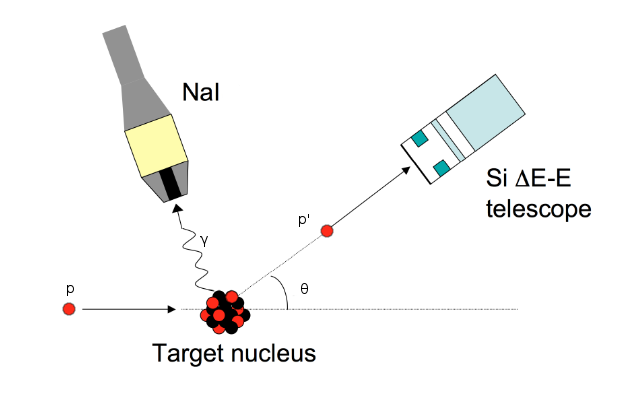
\includegraphics[width=\columnwidth]{nucleus-fixed.png}
    \caption{Our reaction $^{28}\text{Si(p, p')}^{28}\text{Si}^*$ visualised
        with incoming proton, nucleus and the CACTUS and SiRi detectors.}
    \label{fig:28si}
\end{figure}

\section{Method}
\subsection{Experimental Setup}
A cyclotron is a particle accelerator in which a beam of charged particles
is accelerated circularly by a radio frequency (RF) electric field.
The beam is controlled to the circular path by a magnetic field,
that increases the radius of the spiral as the particles are accelerated.
\begin{figure}[h!]
    \centering
    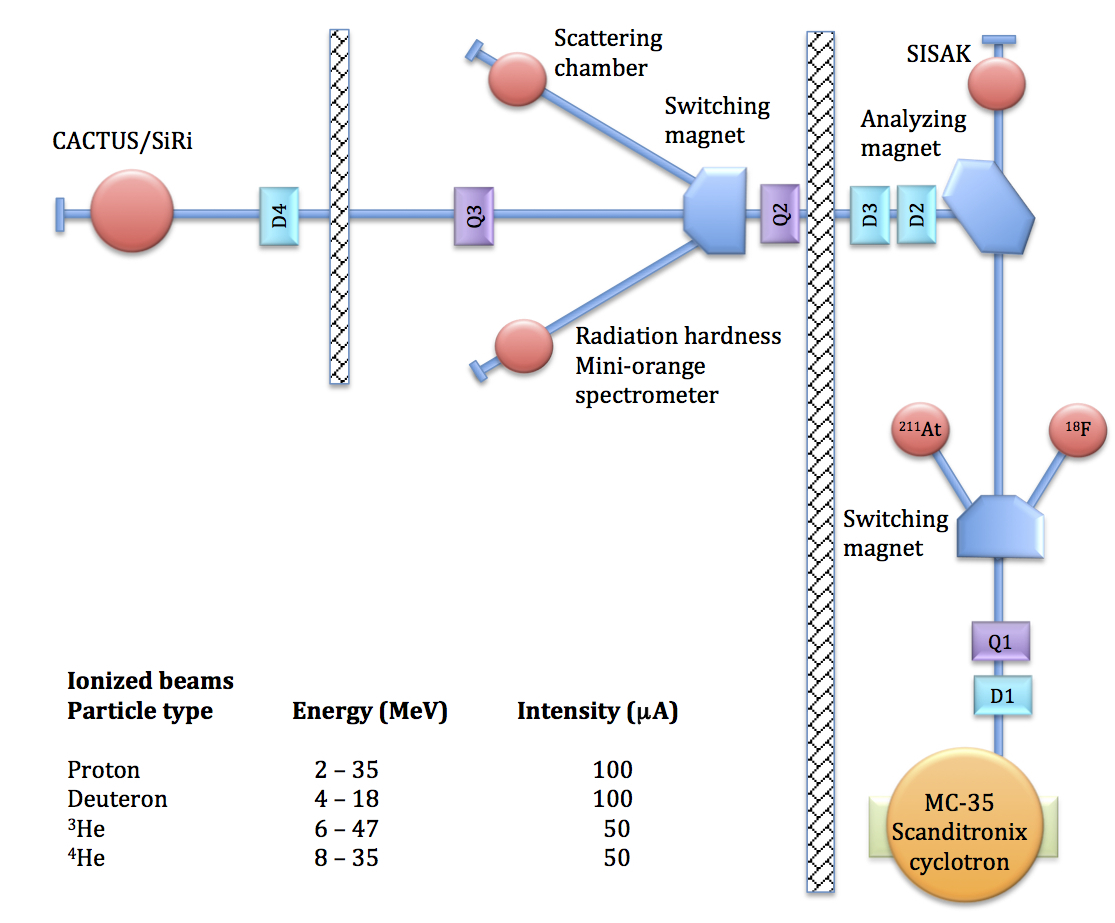
\includegraphics[width=\columnwidth]{ocl-layout.jpg}
    \caption{The accelerator layout used at the OCL.}
    \label{fig:accelerator}
\end{figure}
The experimental setup of the accelerator at OCL is 
explained in figure \ref{fig:accelerator}. 
\begin{figure}[h!]
    \centering
    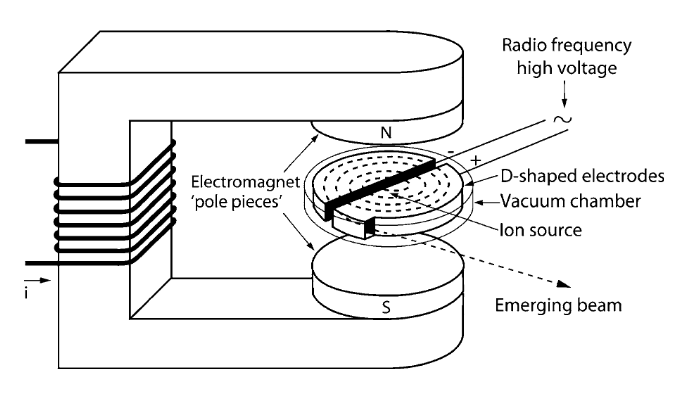
\includegraphics[width=\columnwidth]{cyclotron-schematic-tavernier.png}
    \caption{Schematic representation of a cyclotron [1]. Tavernier}
    \label{fig:cyclotron}
\end{figure}

The particles are accelerated in the bottom right corner in the
cyclotron 
(The principle schematics of a cyclotron can be seen 
in figure \ref{fig:cyclotron}.)
before being shot at our $^{28}\text{Si}$ target nucleus 
in the top left corner.
Around the target, we have placed a \emph{Silicon Ring detector} 
(SiRi, $\Delta E - E$ telescope)
to measure the energy of the proton, and a \emph{CACTUS detector} 
to capture emitted photons from the excited nucleus.

The SiRi detector consists of eight Silicon detectors
assembled in a ring, and each of these is two-parted.
First comes the $\Delta E$ layer, which measures the energy loss,
and then the $E$ layer, which stops the momentum of the particle.
The $E$ layer is significantly deeper than the $\Delta E$,
which was \SI{130}{\micro\meter} in our setup.
In addition, each of the eight Si parts is divided into another
eight strips, used to measure the angle of the incoming particle.

The CACTUS detector consists of 28\footnote{Only 26 of these were 
    working when our data was recorded.}
NaI scintilators, assembled in a ball around the SiRi detector.
Scintillators absorb high-energy electromagnetic waves,
and then re-emit them in the form of photons around the visible spectrum.
This light is then measured by a photomultiplier tube (PMT),
and thus we know the energy of the original ray.

\subsection{Data analysis}
The main goal of this report is to treat the incoming data
from the experiment. This is done using various analysing methods,
which we present in this section.

The data we analyse is mainly the $\Delta E$ and $E$ values measured
by SiRi, and the gamma ray energy from CACTUS in our time window.
These large data files for the events described above,
are filtered using a sorting software,
written in \textit{C++} by (among others) 
Magne Guttormsen at the OCL laboratory.

We will first go through the different parts of the software
used for analysing the data\footnote{The source code can in its entirety
be found at \url{https://github.com/oslocyclotronlab/oslo-method-software},
though we used a modified and primitive version of this code.}.

The main class of the sorting code is in \\
\verb+User_sort.cpp+,
and this script performs the actual sorting.
We modify this code to change the various parameters
like including time gates and gating on excited nucelus states.
To run the sorting code, we have a \verb+Makefile+
that creates the executable \verb+sorting+.
When executed, it checks\\
\verb+<current-experiment>.batch+
for where to locate the data files.
It calls on the gain and shift file \verb+gainshift_525.dat+,
which has the particle, time and detector calibrations.
It also calls \verb+zrange_p.dat+, which containts information
about the protons energy loss during the penetration of the SiRi detector.

\paragraph{Particle Calibration}
To achieve a meaningful result, we first have to calibrate the 
detectors. Our data contains information about the energy
$\Delta E$ lost in the first part of the detector,
and the remaining energy $E$ lost when the particle is stopped.
By plotting the relationship between $\sfrac{E}{\Delta E}$,
we obtain distinct curves, corresponding to a given particle.
These curves are commonly referred to as \textit{bananas}
(see figure \ref{fig:bananas-plain}).

\begin{figure}[H]
    \centering
    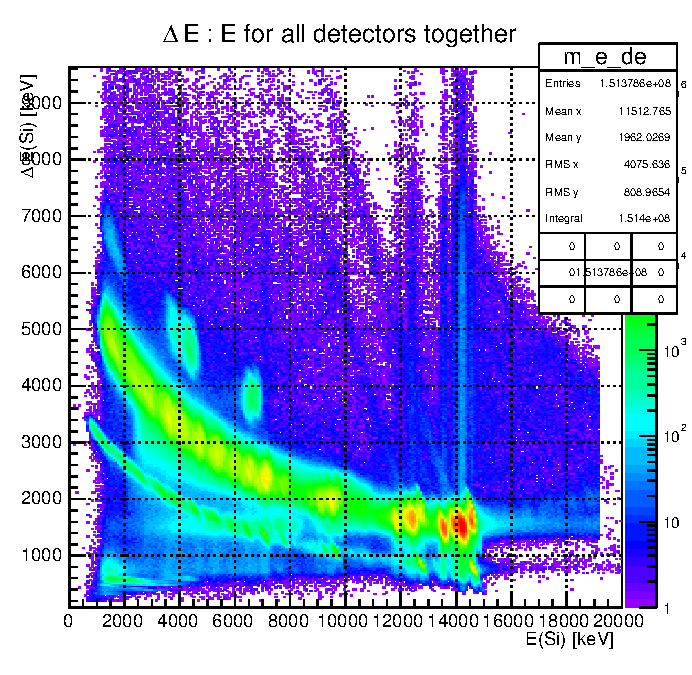
\includegraphics[width=\columnwidth]{/home/alexander/Downloads/Week2/m-e-de-uncalibrated.pdf}
    \caption{The $\sfrac{\Delta E}{E}$ plot showing the result of the }
    \label{fig:bananas-plain}
\end{figure}

The detector setup has eight Si detectors, where each of the detectors
are divided into another eight rings. Each ring corresponds to
an \emph{angle} (of the incoming particle) and thus for a given angle, 
in theory, all of the bananas should look the same.
In the experiment we performed, this is not the case,
and we need to align the detectors accordingly.
By looking at the peaks of the ground-state energy
and the energy of the first excited state in the bananas, we obtain reference
values that we can use to align the detectors.
We measure the $\Delta E$ and $E$ values
and compare with the values we obtained for each ring.

The response of the detectors is appriximately linear
with respect to energy, and thus we can express $\Delta E$ and $E$
on the form
\eq{E(x) &= a_E + b_E x\\
    \Delta E(x) &= a_{\Delta E} + b_{\Delta E} x
}
where $a$ is the energy in the chosen reference channel
(\emph{shift}),
$b$ is the energy of each channel (\emph{gain}) and
$x$ is the channel number. We fit the constants $a_i$ and $b_i$
such that the energy values of the reference peaks of the experiment 
fit the calculated values.
We have performed this calibration for all eight detectors and
their respective eight strips. In total this gives 
64 $\Delta E - E$ pairs that need calibration constants.

\paragraph{Selecting a Reaction}
After having aligned the bananas, 
we must choose the appropriate reaction, which is
called \textit{gating}.
We must gate on the banana corresponding to
this reaction, which can be seen in figure \ref{banana-plain-gated}.
This is done by changing the relevant parameter
(\textit{parameter_thick_range})in \\
\verb+zrange_p.dat+ for the ejected proton,
to the values obtained from the banana we are interested in,
using this as the input in the \verb+.batch+ file
and then sorting again.
Since we know the thickness of the $\Delta E$ detectors,
the experimental data will be centered at $\sim$\SI{130}{\micro\meter}
(we see in figure \ref{de-thickness} that the apparent thickness
corresponds to the actual of the $\Delta E$ detector).

This allows us to find the excitation levels of
the remaining nucleus. We do this by
projecting the coincidence matrix on the $y$-axis,
as seen in figure \ref{fig:excited-states}.

\paragraph{Gamma Calibration}
We must also calibrate the CACTUS detector and the time signals,
and we do this in a similar way to how we did it for the
SiRi detector.
The time signals are not aligned due to differences in
the electronics used to measure the incoming photons.
We have 28 (actually 26) scintillators that we need to align,
and we choose one of these as a reference for the others.
The scintillators register how many counts of gamma rays
that are measured, and we must align the peaks to the reference value.
In a similar manner to the SiRi calibration, we must
also change the shift and gain for the NaI detector in the sorting routine.

To find the input we are interested in, we use \textit{discriminators}.
The CACTUS detector uses \textit{leading-edge discriminators (LEDs)},
which looks at the leading edge of the signal,
and when the threshold is achieved, registers it.
This can lead to variance in the timing, due to the size
of the signal (this is variance is called \textit{walk}).
We adjust for this by doing a curve fitting, and
with the sorting program, correct for the energy dependence
caused by the difference in amplitude of the signal.
The corresponding uncorrected result
is shown in figure \ref{fig:time-uncorrected}.

\begin{figure}[H]
    \centering
    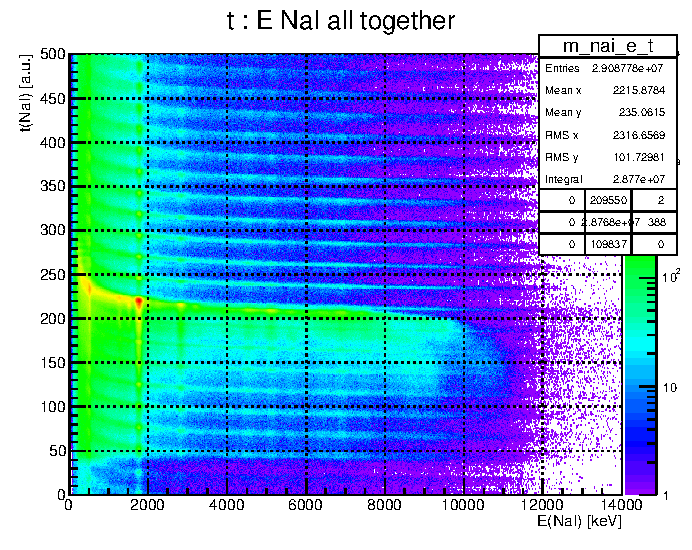
\includegraphics[width=\columnwidth]{/home/alexander/Downloads/week3/m-nai-e-t-corrected.pdf}
    \caption{The plot of the response from all of the 28 (26) NaI detectors, with photon count on the $z$-axis.}
    \label{fig:time-uncorrected}
\end{figure}

\textit{Constant fraction discriminators (CFDs)} does not have this
problem, since they look at a fraction of the incoming
signal, but since they are more expensive, our device
is equipped with LEDs.

After the time signals have been corrected for,
we must locate the reaction that we really want,
which are the gamma rays emitted after the proton has
hit the nucleus. These are called \textit{prompt gammas},
and we say that they are \textit{in coincidence} with the
emitted proton.
We gate on the desired reaction by plotting the number of
counts of gammas vs. the time-aligned channels and then
gate around the prompt peak (we subtract everything around)
so that we obtain only the reaction we wish for.

When we measure the gamma rays there is also one more thing we
must account for, and that is unwanted gamma rays from other 
decaying nucleii.
We have chosen some time windows, but unfortunately
previously excited nucleii might decide to decay during
this window, and unwanted gamma rays from the background 
might interfere with our data.
We deal with the background radiation by starting the experiment
without any reaction, and substract this from the experiment data.
The delayed gamma rays mentioned before can be removed by
gating on these random events and then subtracting the
corresponding values from the experiment data.

\subsection{The Oslo Method}
As we have discussed earlier, the main reason for finding the
coincidence matrix, is to apply the Oslo method.
Using the Oslo method, we can find the \\
\textit{nuclear level density (NLD)}
$\rho$ and the \textit{gamma strength function ($\gamma$SF)} 
$\tau$ in one experiment.
This lets us calculate the probability $P$ of our reaction,
due to the proportionality realtion
\eq{P(E_x,E_\gamma)\propto \tau(E_\gamma)\cdot\rho(E_x-E_\gamma)}

The method consists of three steps
\begin{enumerate}
    \item Unfolding the gamma ray spectrum.
    \item Extracting the first generation gamma rays.
    \item Extracting $\rho$ and $\tau$.
\end{enumerate}

where the last step is a too large a task to be done
in this project.

\paragraph{Unfolding of the Coincidence Matrix}
Unfolding is the act of removing unwanted interactions with
the CACTUS detector. 
When we detect gamma rays, we
will not only observe peaks at the desired energy level,
but rather a spectrum like shown in figure \ref{fig:peaks}.

We will see compton scattering, which will show like an
edge-like form. Pair-production, where an electron and a
positron is created, and one or both might escape,
shows like one or two sharp peaks. 
The last effect, which is the one we want to be large,
is the photoelectric effect. This will show as a peak
(which is also contributed by the two other effects)
at the energy we want. The pair-production energies
are respectively \SI{511}{\kilo\electronvolt} 
and \SI{1022}{\kilo\electronvolt} lower than this peak,
which corresponds to one and two times the electron rest-mass.

The unfolded matrix is found by
\eq{f = Ru}

where $R$ is a response matrix that contains information
about the response of the detector.
Finding this matrix is not part of our project, but has been done for us.
Unfolding the matrix, removing the parts we are not interested in,
and then refolding it, gives us the result in figure \ref{fig:unfolded}.

\begin{figure}[H]
    \centering
    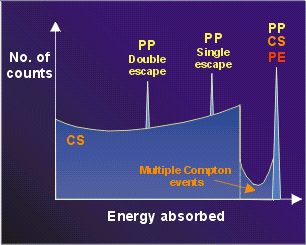
\includegraphics[width=\columnwidth]{/home/alexander/UiO/fys4180/final-project/figures/escape-peak.png}
    \caption{A typical spectrum of detected energies in a gamma ray detector.}
    \label{fig:peaks}
\end{figure}


\paragraph{Multiplicity}
During our measurement of the gamma rays from the excited nucleus,
we count how many that hits our detector in time period.
The count doesn't exclude the ones that come from a nucleus
that has not emitted all its energy in one ray, and thus
sends out more than one photon for each reaction.
We call the first photon to be emitted from an excited nucleus
\textit{first generation} gamma rays. In our analysis,
we want to exclude all the non-first generation photons from
our count, because they will skew the probability of going
from one state to another.
This is visualised in figure \ref{fig:squiggly-states}.

We therefore introduce a quantity called the \textit{multiplicity}
$\langle M \rangle$.
It is defined as the average number of photons emitted by
an excited nucleus with energy $E_x$.
Here we present two ways of obtaining this quantity
\equ{\langle M \rangle =\frac{E_x}{\langle E_\gamma\rangle}\label{eq:M1}}
and the iterative \textit{first generation} method
\equ{\langle M \rangle = k\cdot \frac{N_c}{N_s}\label{eq:M2}}
where $\langle\cdot\rangle$ denotes the average value of the quantity.

In equation \ref{eq:M2}, $k$ is some unknown constant that we can
find by finding the multiplicity using equation \ref{eq:M1}.
$N_s$ and $N_c$ are the spectra of the banana plots 
(the \textit{singles} spectrum) and of the coincidence of the energy of
the proton and the gamma ray (the \textit{coincidence} spectrum).

\begin{figure}[H]
    \centering
    \begin{tikzpicture}
        \draw[thick,->] (0,0)  -- (7,0) node(xline)[right] {$E_{gs}$};
        \draw[thick,->] (0,0) -- (0,7) node(yline)[above] {$E_x$};
        \draw[] (0,3) -- (7,3) node[right] {$E_1$};
        \draw[] (0,5) -- (7,5) node[right] {$E_2$};
        \draw[] (0,6) -- (7,6) node[right] {$E_3$};
        \draw[->,line join=round,
            decorate, decoration={
            snake,
            segment length=10,
            amplitude=1.5,post=lineto,
            post length=2pt
        }, red] (1,6) -- (1,0);

        \draw[->,line join=round,
            decorate, decoration={
            snake,
            segment length=10,
            amplitude=1.5,post=lineto,
            post length=2pt
        }, red] (1.5,6) -- (1.5,3);
        \draw[->,line join=round,
            decorate, decoration={
            snake,
            segment length=10,
            amplitude=1.5,post=lineto,
            post length=2pt
        }, cyan] (1.5,3) -- (1.5,0);

        \draw[->,line join=round,
            decorate, decoration={
            snake,
            segment length=10,
            amplitude=1.5,post=lineto,
            post length=2pt
        }, red] (2,6) -- (2,5);
        \draw[->,line join=round,
            decorate, decoration={
            snake,
            segment length=10,
            amplitude=1.5,post=lineto,
            post length=2pt
        }, cyan] (2,5) -- (2,0);

        \draw[->,line join=round,
            decorate, decoration={
            snake,
            segment length=10,
            amplitude=1.5,post=lineto,
            post length=2pt
        }, red] (2.5,6) -- (2.5,5);
        \draw[->,line join=round,
            decorate, decoration={
            snake,
            segment length=10,
            amplitude=1.5,post=lineto,
            post length=2pt
        }, cyan] (2.5,5) -- (2.5,3);
        \draw[->,line join=round,
            decorate, decoration={
            snake,
            segment length=10,
            amplitude=1.5,post=lineto,
            post length=2pt
        }, green] (2.5,3) -- (2.5,0);

        \draw[->,line join=round,
            decorate, decoration={
            snake,
            segment length=10,
            amplitude=1.5,post=lineto,
            post length=2pt
        }, red] (3.5,5) -- (3.5,0);

        \draw[->,line join=round,
            decorate, decoration={
            snake,
            segment length=10,
            amplitude=1.5,post=lineto,
            post length=2pt
        }, red] (4,5) -- (4,3);
        \draw[->,line join=round,
            decorate, decoration={
            snake,
            segment length=10,
            amplitude=1.5,post=lineto,
            post length=2pt
        }, cyan] (4,3) -- (4,0);

        \draw[->,line join=round,
            decorate, decoration={
            snake,
            segment length=10,
            amplitude=1.5,post=lineto,
            post length=2pt
        }, red] (5,3) -- (5,0);
    \end{tikzpicture}
    \caption{Here we see the different paths a gamma ray can go from its
        start energy (excited state) down to the ground state. The first
        generation photons are the red arrows.}
    \label{fig:squiggly-states}
\end{figure}

\section{Results}

In figure \ref{fig:bananas-plain} we saw the uncalibrated banana,
and in figure \ref{fig:bananas-plain-calibrated} we present
the particle calibrated result, that is after we have calibrated
the SiRi detector. We see that the banana (or the reaction)
we are interested is clearly visible, with less noise and other reactions.

\begin{figure}[H]
    \centering
    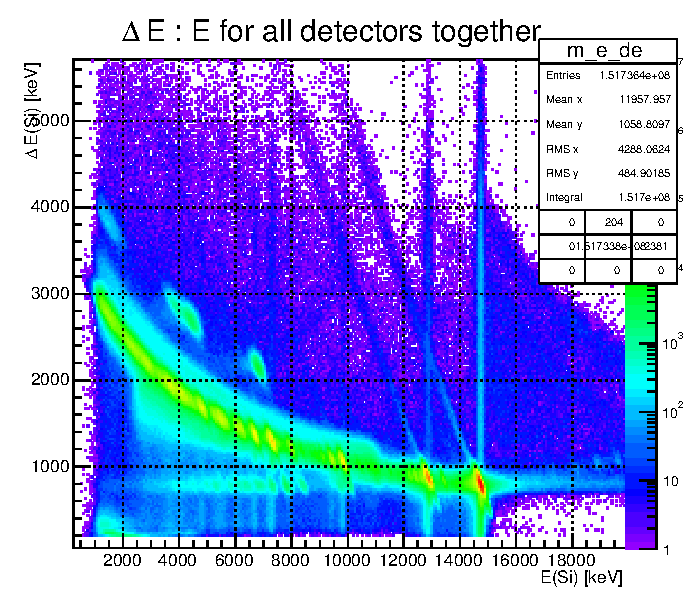
\includegraphics[width=\columnwidth]{/home/alexander/Downloads/Week2/m-e-de-calibrated.pdf}
    \caption{The $\sfrac{E}{\Delta E}$ plot after calibration of the SiRi detector.}
    \label{fig:bananas-plain-calibrated}
\end{figure}

We gated on the banana of our reaction, which means we cut away
all of the irrelevant data. This
is shown in figure \ref{bananas-gated}.

\begin{figure}[H]
    \centering
    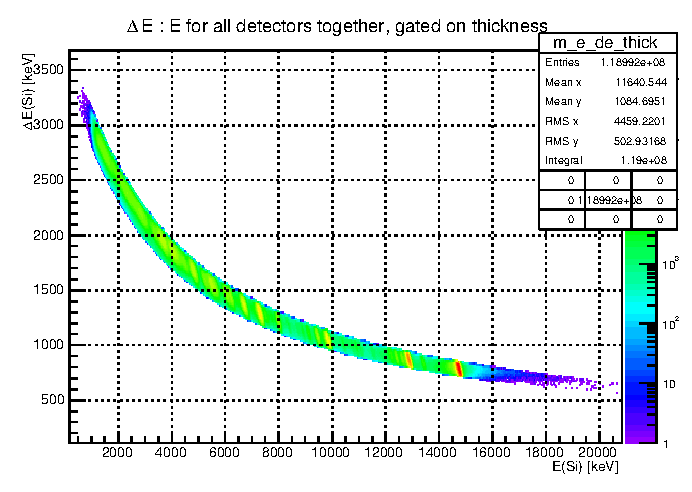
\includegraphics[width=\columnwidth]{/home/alexander/UiO/fys4180/final-project/figures/m-e-de-thick.pdf}
    \caption{Gating on a calibrated banana. This shows that we remove
    the data which we are not interested in.}
    \label{fig:bananas-gated}
\end{figure}

We projected the calibrated coincidence matrix on the $y$-axis
to visualise the excited states of the nucleus after
calibrating the gamma ray detector. This is shown in
\ref{fig:excited-states}, and we compare the results
with known excitation values values of Silicon-28 given by the 
\textit{National Nuclear Data Center (NNDC)}
website\footnote{\url{http://www.nndc.bnl.gov/chart/getdataset.jsp?nucleus=28SI&unc=nds}}. 
We see that there are some peaks which doesn't correspond
to the values in table \ref{tab:excited-nucleii},
so we see that at this point 
there is still some stuff that has not been corrected.

\begin{figure}[H]
    \centering
    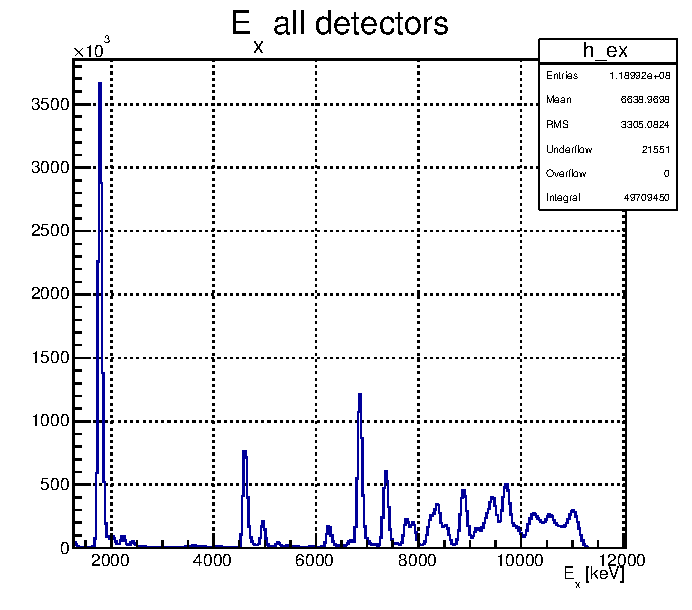
\includegraphics[width=\columnwidth]{/home/alexander/Downloads/Week2/h-ex-calibrated-zoom.pdf}
    \caption{Projection of the coincidence matrix on the $y$-axis
    for the excitation energy $E_x$ vs. the number of photons counted.
    We see that the first six peaks corresponds to the known
    values for the excitation values of $^{28}\text{Si}$.}
    \label{fig:excited-states}
\end{figure}

\begin{table}[h!]
    \centering
    \begin{tabularx}{\columnwidth}{| X | X | X | X |}
        \hline
        $E_x$ [keV] & 0.0 & 1779.030 & 4617.86 \\ \hline
        & 4979.92 & 6276.2 & 6690.74\\
        \hline
    \end{tabularx}
    \caption{The first six excitation levels of $^{28}\text{Si}$ 
        from NNDC.}
    \label{tab:excited-nucleii}
\end{table}

The next step was to calibrate CACTUS time signals,
and we have previously seen that the energy is time dependent.
In figure \ref{fig:time-corrected} we see how the correction of the
timing results in a linear response in time,
versus the uncalibrated one in figure \ref{fig:time-uncorrected}.

\begin{figure}[H]
    \centering
    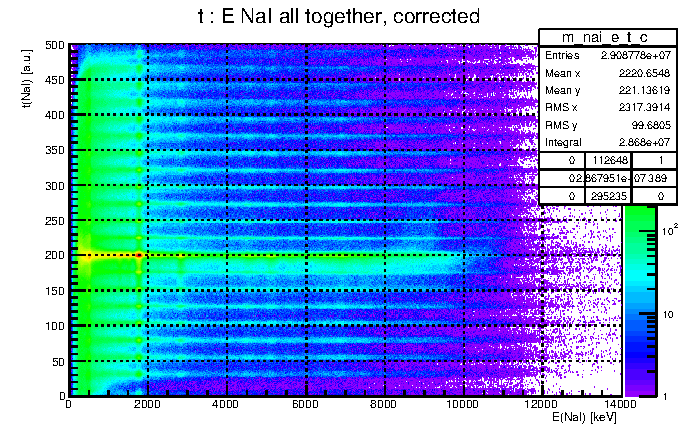
\includegraphics[width=\columnwidth]{/home/alexander/Downloads/week3/m-nai-e-t-corrected-fit.pdf}
    \caption{Plot of the corrected energy of all the detectors from CACTUS 
        vs. the time channels, with a curve fitting.}
    \label{fig:time-corrected}
\end{figure}

After we have done all of our calibrations, we return to our
primary objective -- obtaining the calibrated coincidence matrix.
The result is shown in figure \ref{fig:coincidence-corrected-final}

\begin{figure}[H]
    \centering
    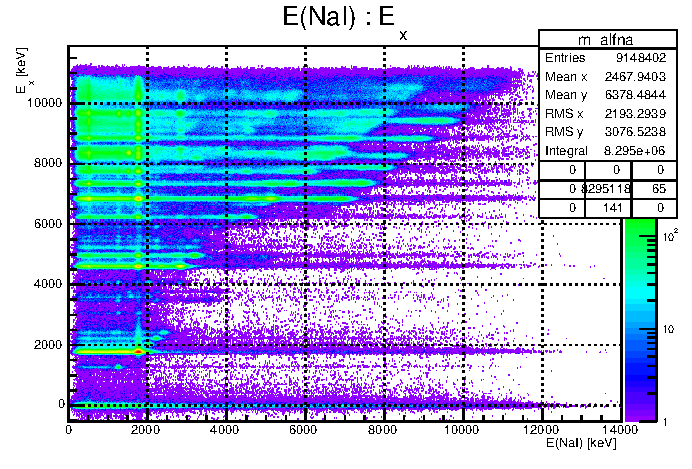
\includegraphics[width=\columnwidth]{/home/alexander/UiO/fys4180/final-project/figures/m-alfna-week2.pdf}
    \caption{The coincidence matrix after corrections of both the SiRi detector and the CACTUS detector as well as removal of the background radiation
        and random coincidences.}
    \label{fig:coincidence-corrected-final}
\end{figure}

The reason we wanted to obtain the corrected coincidence matrix was
to perform the Oslo method. The second step in the method was
to unfold the matrix to focus on the photoelectric effect contributions.
We therefore present the final result -- the unfolded and refolded
coincidence matrix, with the lower diagonal removed.
See figure \ref{fig:refolded-matrix}

\begin{figure}[H]
    \centering
    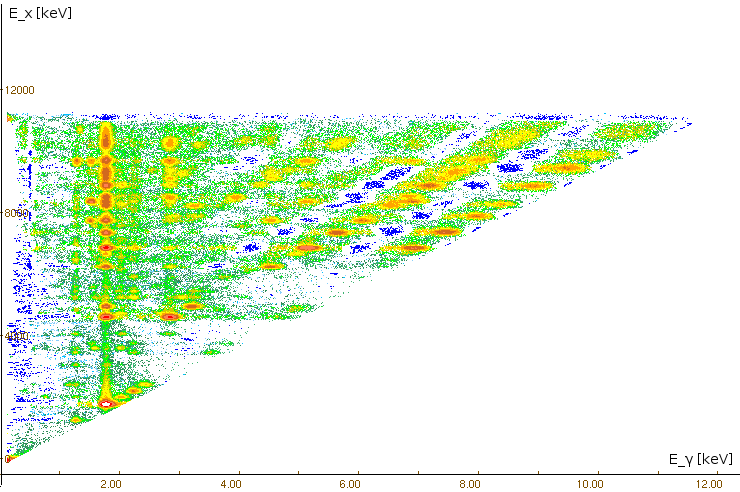
\includegraphics[width=\columnwidth]{/home/alexander/UiO/fys4180/final-project/figures/alfna-no-background.png}
    \caption{The final result. The corrected coincidence matrix callibrated,
    and unfolded.}
    \label{fig:refolded-matrix}
\end{figure}

\section{Conclusion}
In this report we have looked at the reaction of\\ 
$^{28}\text{Si(p, p')}^{28}\text{Si}^*$ and applied various
analysing methods to achieve the main goal of
obtaining a calibrated coincidence matrix that we
can apply the Oslo method to.
This is an important part in extracting the nuclear density levels
and the gamma-ray strength function to eventually find the 
probability $P(E_x,E_\gamma)$
of the reaction, which would have been the next step in the process. 

While doing this, we have learned about the cyclotron,
and the particle accelerator at the OCL, and the amount of work that
has to be done after doing the actual experiment to extract
useful information.

I would like to thank Lucia Crespo Campo for supervising the project
and the OCL for the educational experience.
\end{document}
